\documentclass[a4paper]{article}
\usepackage[utf8]{inputenc}
\usepackage{amsmath}
\usepackage{graphicx}
\usepackage{float}
\usepackage{color}
\usepackage[dvipsnames]{xcolor}
\usepackage{tabto}

\title{Report\\Numerical Simulation of Beam Propagation including Error Convergence Analysis}
\date{15-05-2018}

\author{Prepared by: Nicolae Cadin \\Supervised by: Ramon Springer}




\begin{document}
	
	
	\pagenumbering{gobble}
	\maketitle
	\newpage
	\tableofcontents	

	\pagenumbering{arabic}
%	\setlength\parindent{0pt}
	
	\newpage
	\section{Introduction}
	Beam propagation in media is of high interest for scientists and also for industrial purposes. 
	In this report beam propagation will be simulated, problems will be discussed. The purpose of the project is to compare numerical method and analytical solution. Convergence of used numerical method is to be shown. For the simplicity simulation of beam propagation is done in free space, linear medium, at zero incident angle, so to fit the scope of mini-project, later on can be extended for more sophisticated cases.
	\subsection{Analytical solution}
	To better analytically understand propagation of beam in space we should solve Helmholz Equation.
	\begin{center}
		$(\nabla^2+k^2)E = 0$		
	\end{center}
	This equation generally holds for electromagnetic wave, hence for electric and magnetic field components, for simplicity we chose electric field $E$. Here $k$ is wave number and is equal to $2\pi n/\lambda$, where $\lambda$ is wavelength, $n$ is refractive index of the medium (here we assume it to be equal to 1). As assumption we consider that our wave propagates in $z$ direction and electric field can be represented in next form.
	\begin{center}
		$E(x,y,z)=u(x,y,z)e^{-ik_oz}$
	\end{center}
	$u$ is complex function which describes non-plane part of the beam. Substituting our ansatz into Helmholtz equation in cartesian coordinates and doing some simplifications we get.

	\[\frac{\partial^2 u}{\partial x^2}+ \frac{\partial^2 u}{\partial y^2}+ \frac{\partial^2 u}{\partial z^2} - 2ik_o\frac{\partial u}{\partial z}+(k^2-k_o^2)u=0\]
	Using paraxial approximation we see that third term is smaller than others, therefore can be neglected, as result we get following equation.
	
	\begin{equation}\label{eq:1}
	\frac{\partial^2 u}{\partial x^2}+ \frac{\partial^2 u}{\partial y^2} - 2ik_o\frac{\partial u}{\partial z}+(k^2-k_o^2)u=0
	\end{equation}
	Solving this differential equation we find $u$, hence we find $E$. We assume that $k = k_o$, therefore solution for two dimensional case, where wave propagates in z-direction and oscillates in xz plane is,
	\begin{equation}\label{eq:2}
	E(x,z)=E_o\bigg(\frac{w_o}{w(z)}\bigg)^{\frac{1}{2}}exp\bigg(\frac{x^2}{w(z)^2}\bigg)exp\bigg(-i\Big(k_oz+k_o\frac{x^2}{2R(z)}-\phi(z)\Big)\bigg)
	\end{equation}
	where $w(z)$ is beam radius, $w_o = w(0)$ is beam waist, $E_o$ is electric field amplitude, $R(z)$ is beam curvature, $\phi$ is Gouy phase. Their explicit mathematical formula can be found in the Table \ref{tab:Table1}. This electric field formula will be later used as reference to numerical solution. From here intensity can be calculated, $I = \frac{\epsilon _o c n_o}{2}|E_z|^2$. Implementation of analytical solution can be found it Appendix A. 
	
%	\[w(z)= w_o\sqrt{1+\Big(\frac{z\lambda}{\pi w_o^2}\Big)^2}\]
%	\[R=z\bigg[1+\Big(\frac{\pi w_o^2}{z\lambda}\Big)^2\bigg]\]
%	\[\phi(z)=arctan\Big(\frac{z\lambda}{\pi w_o^2}\Big)\]

	\begin{table}[h!]
		\begin{center}
			\begin{tabular}{c| c| c} % <-- Alignments: 1st column left, 2nd middle and 3rd right, with vertical lines in between
				\textbf{Beam Radius} & \textbf{Beam Curvature} & \textbf{Gouy phase}\\
				\hline
				&&\\
				$w(z)= w_o\sqrt{1+\Big(\frac{z\lambda}{\pi w_o^2}\Big)^2}$ & $R=z\bigg[1+\Big(\frac{\pi w_o^2}{z\lambda}\Big)^2\bigg]$ & $\phi(z)=arctan\Big(\frac{z\lambda}{\pi w_o^2}\Big)$\\
			\end{tabular}
			\caption{\label{tab:Table1} Auxiliary formulas to equation \ref{eq:2}.}
		\end{center}
	\end{table}
	
	\subsection{Numerical solution}
	For one dimensional case Equation \ref{eq:1} can be rewritten in the following form.
	\begin{equation}\label{eq:3}
	2ik_o\frac{\partial u}{\partial z}=\frac{\partial^2 u}{\partial x^2}+(k^2-k_o^2)u
	\end{equation}
	To simulate light beam propagation Beam Propagation Method (BPM) is used. BMP is a discretization of formula (\ref{eq:3}), formula should be discretized for z-component and x-component. For beginning let's do discretization only for z component, our equation will get following form.
	\[2ik_o\frac{u^{l+1}-u^l}{\Delta z}=\frac{\partial^2 u^l}{\partial x^2}+(k^2-k_o^2)u^l\]
	Index $l$ denotes the order of grid points in z-direction. This finite difference scheme is known as {\bf forward difference}. However after discretization of x-component numerical instability can be seen. There is another alternative where order of grid point is taken one step in advance, this method is called {\bf backward difference}
	\[2ik_o\frac{u^{l+1}-u^l}{\Delta z}=\frac{\partial^2 u^{l+1}}{\partial x^2}+(k^2-k_o^2)u^{l+1}\]
	Neither this scheme shows good stability, however the combination of these two solves instability problem. These method is called {\bf Crank-Nicolson} method.
	\[2ik_o\frac{u^{l+1}-u^l}{\Delta z}=(1-\alpha)\frac{\partial^2 u^l}{\partial x^2}+(1-\alpha)(k^2-k_o^2)u^l+\alpha \frac{\partial^2 u^{l+1}}{\partial x^2}+\alpha(k^2-k_o^2)u^{l+1}\]
	$\alpha$ here shows interest of which difference we want higher contribution, usually is set to 1/2. Then Crank-Nicolson scheme gets next form.
	\[2ik_o\frac{u^{l+1}-u^l}{\Delta z}=\frac{1}{2}\bigg(\frac{\partial^2 u^l}{\partial x^2}+(k^2-k_o^2)u^l\bigg)+\frac{1}{2}\bigg(\frac{\partial^2 u^{l+1}}{\partial x^2}+(k^2-k_o^2)u^{l+1}\bigg)\]
	Now discretization of x-component can be performed.

	\begin{equation*}
	\begin{split}
	2ik_o\frac{u_j^{l+1}-u_j^l}{\Delta z}=\frac{1}{2}\bigg(&\frac{u_{j-1}^l-2u_j^l+u_{j+1}^l}{\Delta x^2}+(k^2-k_o^2)u_j^l\bigg)+\\
	& \frac{1}{2}\bigg(\frac{u_{j-1}^{l+1}-2u_j^{l+1}+u_{j+1}^{l+1}}{\Delta x^2}+(k^2-k_o^2)u_j^{l+1}\bigg)
	\end{split}
	\end{equation*}
	$j$ index denotes the order of grid points in x-direction. Such discretization can be rewritten and later solved using tridiagonal matrix algorithm or so called {\bf Thomas algorithm}. 
	\[2ik_o\frac{u^{l+1}-u^l}{\Delta z}=\frac{1}{2}\bigg(L_hu^{l}+L_hu^{l+1}\bigg)\]
	$L_h$ is spacial discretization operator for one dimensional case and is numerically defined in Thomas algorithm as 

	\setlength\arraycolsep{-4.5pt}
	\[ L = \frac{1}{\Delta x^2}\begin{bmatrix}
    -2+(k^2-k_o^2)\Delta x^2& 1& 0& &\dots& & 0 \\
    1 & -2+(k^2-k_o^2)\Delta x^2 & 1& &\dots& & 0 \\
    0 &     1& -2+(k^2-k_o^2)\Delta x^2 & & & & 0 \\
    \vdots & \vdots & \vdots & &\dots& & \vdots \\
    0& 0& 0& && &     -2+(k^2-k_o^2)\Delta x^2
	\end{bmatrix}\]
	
	
	\noindent From here doing simple mathematical rearrangement we can write previous equation in the following form.
		\[u^{l+1} = \bigg(I-\frac{\Delta z}{4ik_o}L_h\bigg)^{-1}\bigg(I+\frac{\Delta z}{4ik_o}L_h\bigg) u^l\]
	Here $I$ is identity matrix, which has the same size as tridiagonal matrix $L$. We can notice that this is iterative process, in our particular case we instantiate $u^{l=0}$ at $z = 0$ to Gaussian function, in another words $u(x,z=0)= E_oexp\big(-\frac{x^2}{w_o^2}\big)$. Implementation of numerical solution can be found in Appendix B
	
	\subsubsection{Absorbing Boundary Condition}
	Implementing numerical method, wave approaching boundary will be reflected, this happens due to the nature of numerical algorithm. Physically this can be interpreted as insertion of mirror at the boundary. Reflection at the boundaries can be prevented introducing absorption, such method is called absorbing boundary condition(ABC). One such way is to add a complex part to refractive index, refractive index becomes $\tilde{n} = n+i\kappa$. $\kappa$  is absorption index, it should increase gradually slowly, fast increase can again cause reflection. Absorption index is designed to have parabolic increase and can be expressed in following way.
	\[\kappa(x)=\kappa_{max}\bigg(\frac{x-l/2+\delta}{\delta}\bigg)^2, x\bigg[\frac{l}{2},\frac{l}{2}-\delta\bigg];\]
	\[\kappa(x)=\kappa_{max}\bigg(\frac{l/2+\delta-x}{\delta}\bigg)^2, x\bigg[-\frac{l}{2}+\delta,-\frac{l}{2}\bigg];\]
	Here, $\kappa_{max}$ is maximum value of absorption index to which absorption index as function of x can increase, $l$ is the width of our computational domain, in our case will be corresponding to range of x, $\delta$ is a part of total width where absorption will be introduced, geometry of introduced absorption can be seen in Figure \ref{fig:Absorption}. It is important to notice that ABC do not change along z-direction. The function $\kappa (x)$ is show in Figure \ref{fig:Absorption}.
	\begin{figure}[h!]
		\centering 
		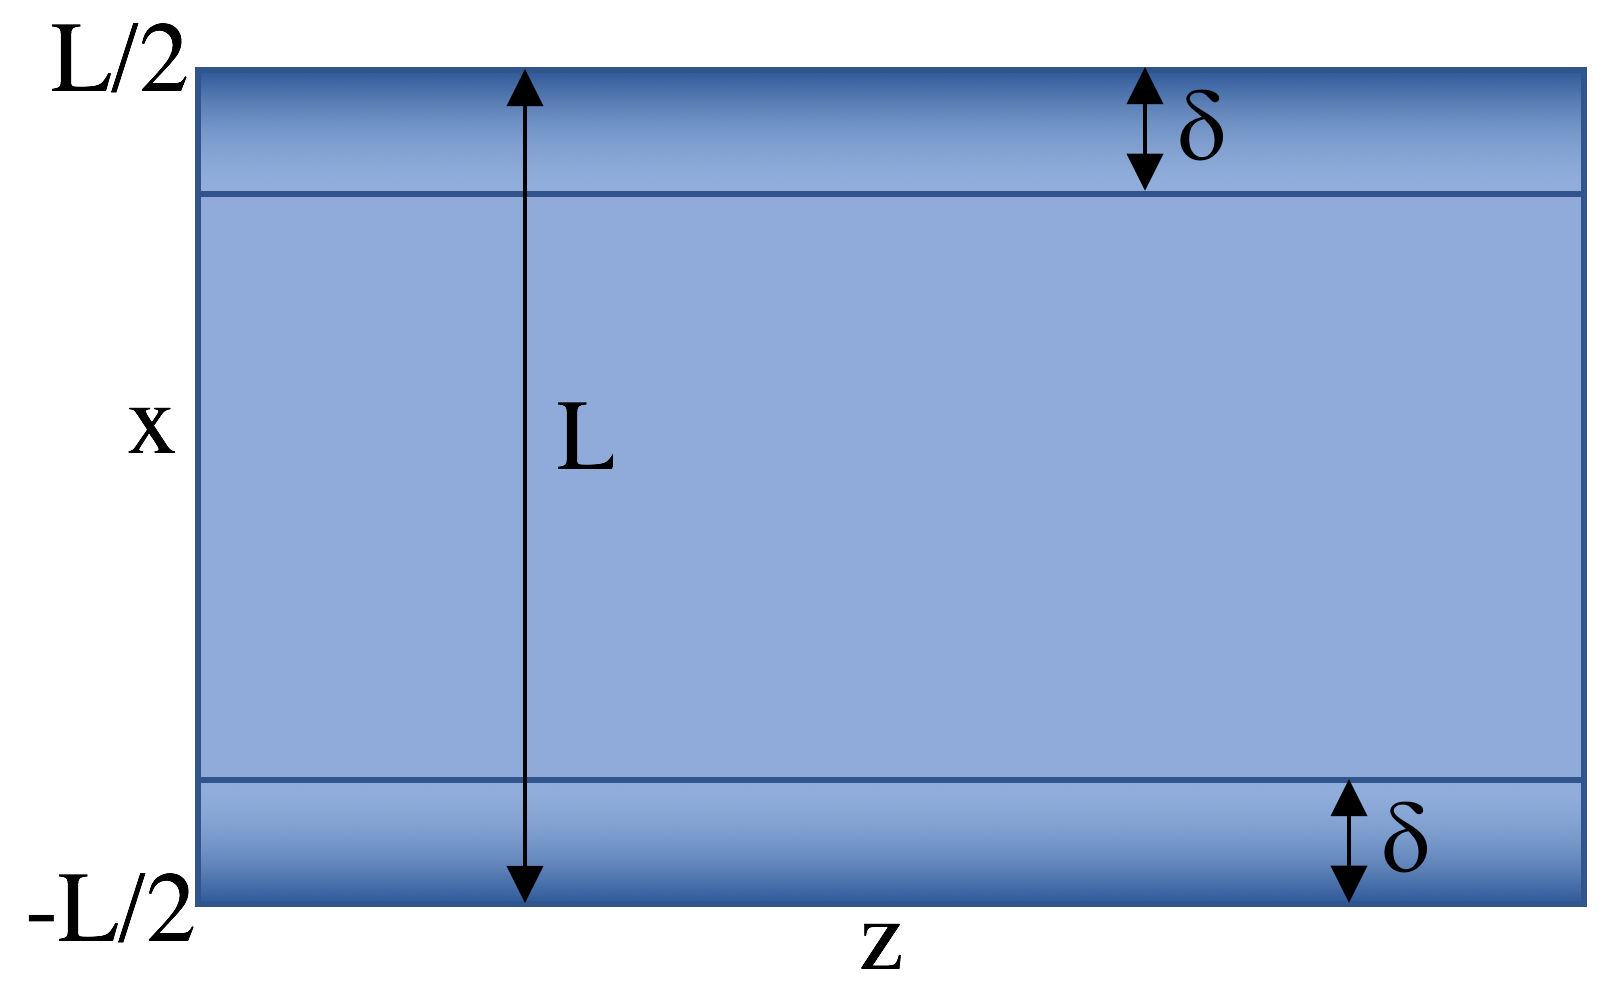
\includegraphics[width=0.5\textwidth]{sketchN1.png}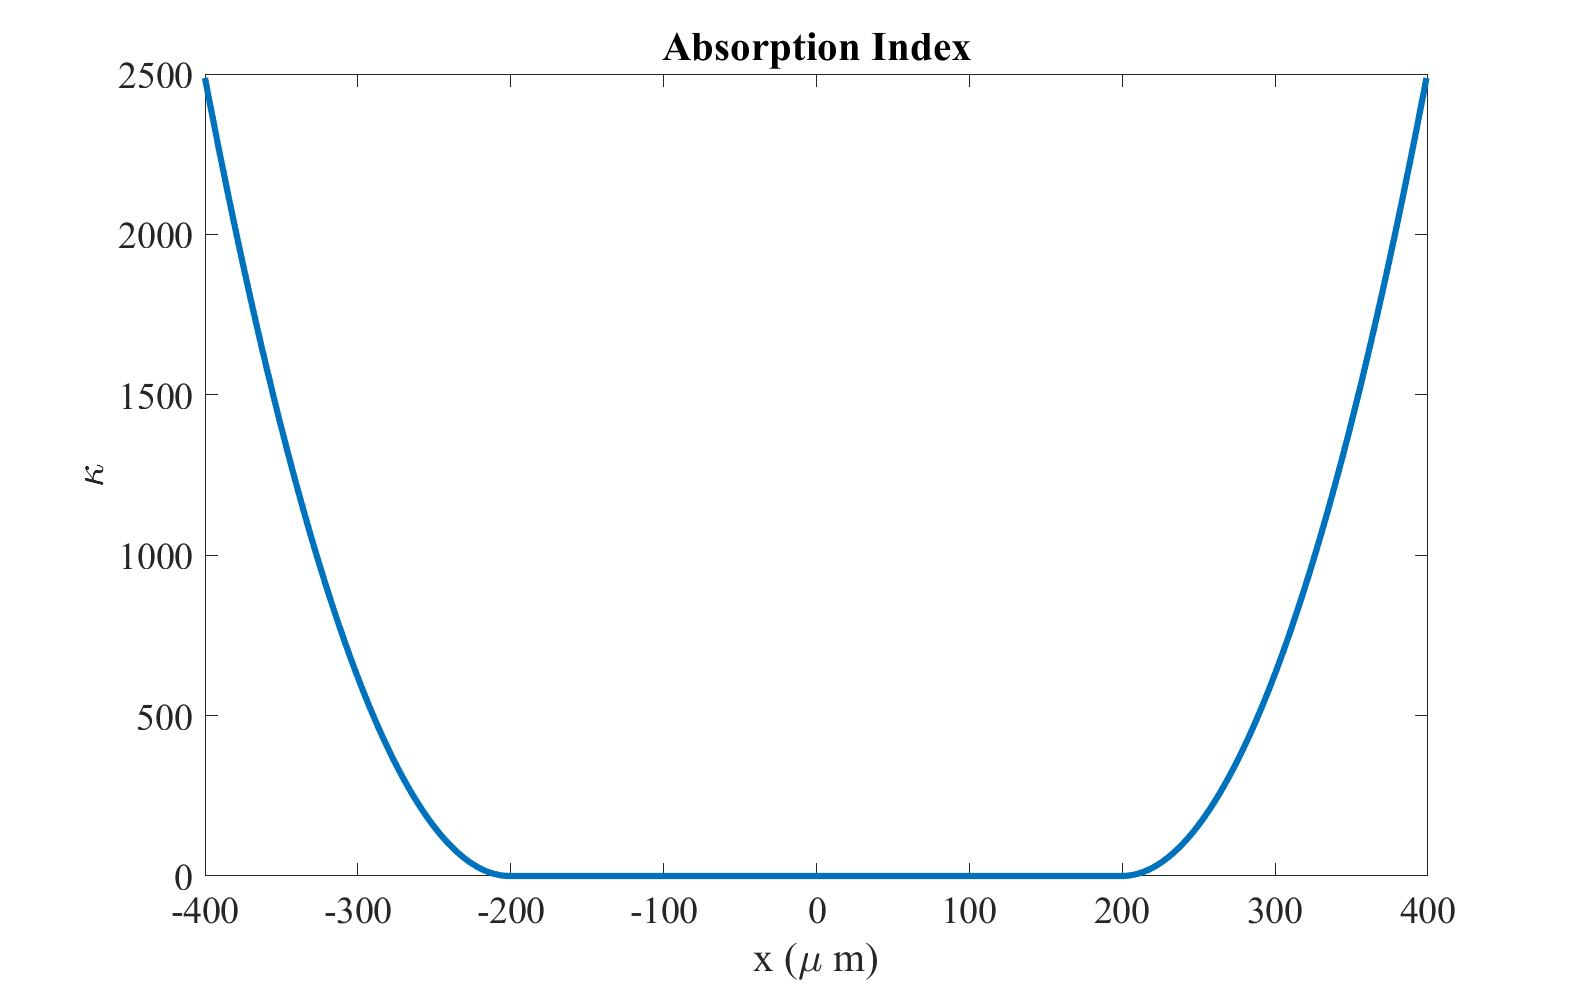
\includegraphics[width=0.5\textwidth]{N2.jpg}
		\caption{\label{fig:Absorption}Absorption boundary, figure on the right shows the geometry of absorbed boundary, appropriate $\delta$ can be chosen during simulation time, figure on the left shows function absorption index $\kappa$ $ (x) $ and its change along x-direction.}
	\end{figure}
	\subsubsection{Error convergence}	
	In order to assess the accuracy of the numerical method, error is calculated. Error is a difference between numerical and analytical electric field and can be calculated using different norms. There is fixed relation between number of grid point and total error, if one increases the number of grid points, error is expected to decrease. If number of grid points is increased $2^n$ times, error should decrease $2^{-n}$ times, $n$ is integer number which also tells about order of error convergence.
	\[||Error||_2 = \frac{1}{\text{{\it Number of grid points}}}\sqrt{\sum\limits_{i=1}^n (E_{\text{\it z numerical}}-E_{\text{\it z analytic}})^2 }
	\]
	\[
	||Error||_\infty = (E_{\text{\it z numerical}}-E_{\text{\it z analytic}})_{maximum}
	\]
	\[ ||Error||_{\text{\it at particular point}} = \text{\it Error at any particular physical point is recorded}
	\]
	\newpage
	\section{Results}
	Numerical algorithm and analytical solution were both implemented and compared, results can be seen in Figure \ref{fig:Results}. In first row depicts Crank-Nicolson numerical method, second row shows analytical solution, first and second columns show real component of electric field and intensity of light consequently. Parameters of laser beam in our case are: z-meshsize = x-meshsize  = 1 $\mu m$, wavelength ($\lambda$) = 20 $\mu m$, waist ($w_o$) = 30 $\mu m$, refractive index ($n_o$) = 1.	
	\begin{figure}[h!]
		\hspace{-30mm}
		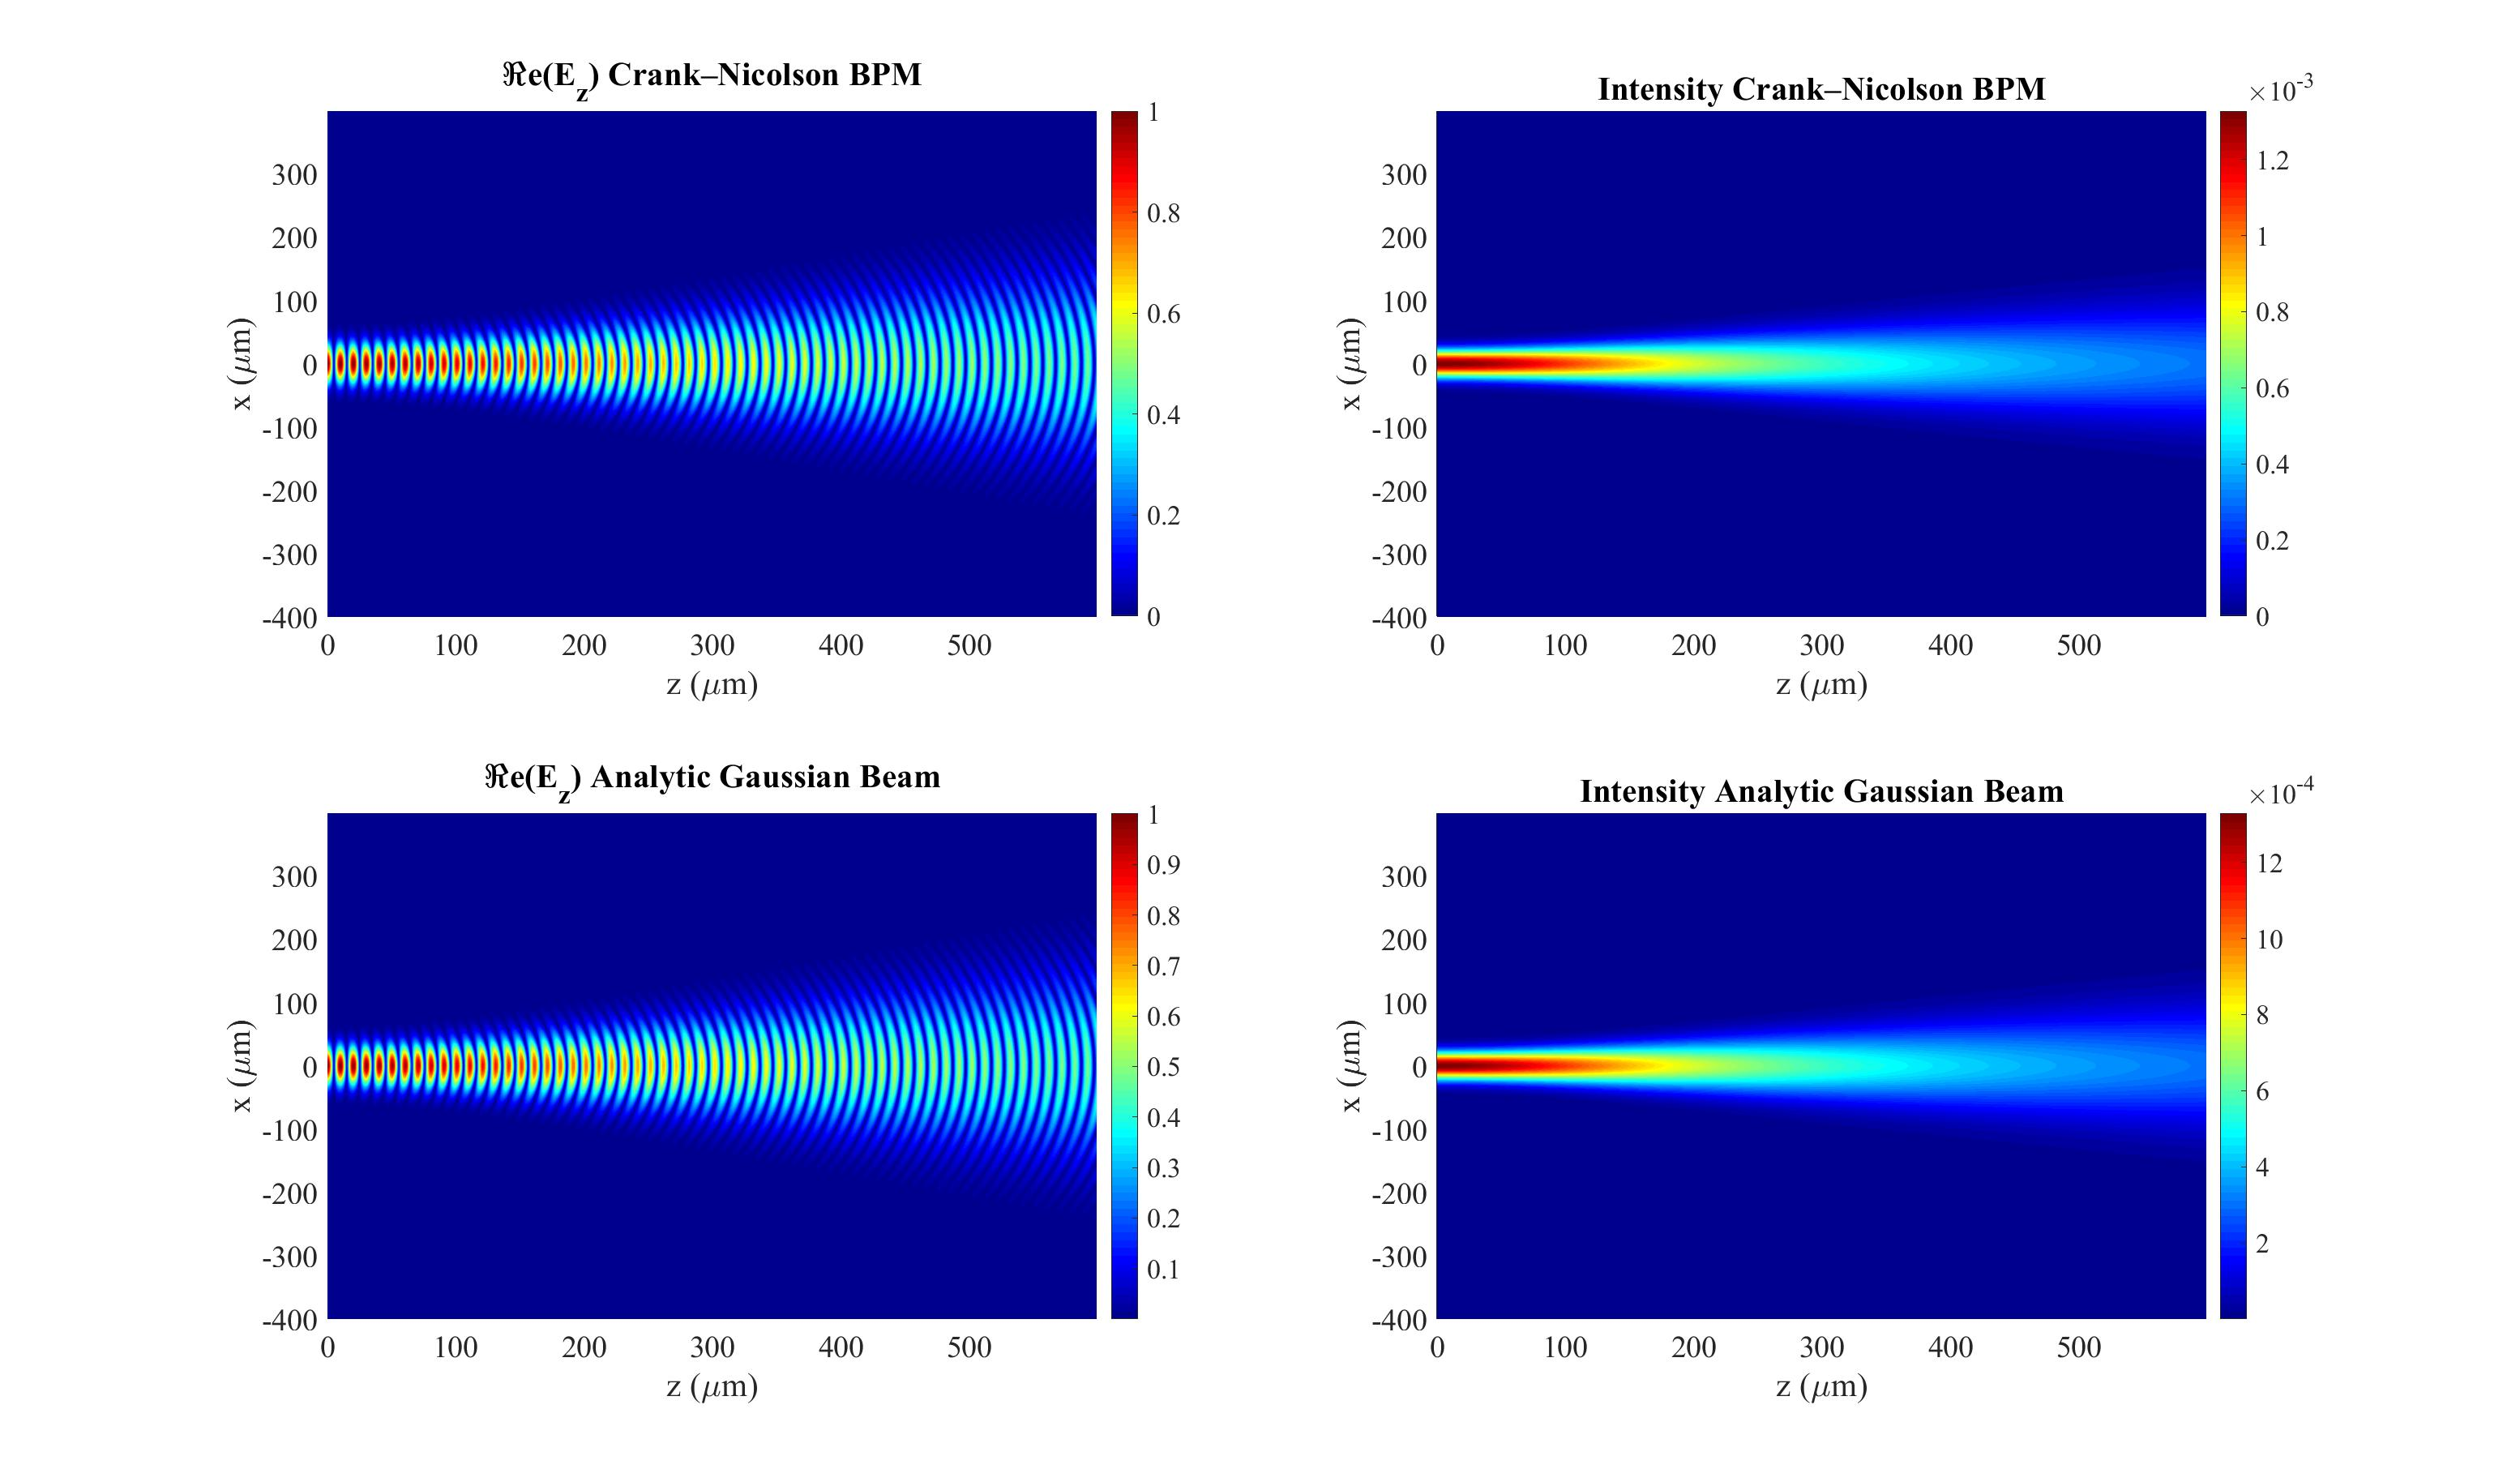
\includegraphics[width=1.5\textwidth]{N1.jpg}
		\caption{\label{fig:Results}Comparison of two methods.}
%		\centering
	\end{figure}
	\subsection{Absorption Boundary Condition}
	In this section we show the results of applied ABC. In Figure \ref{fig:Absorption2} the necessity of applying ABC can be seen. In the figure on the left no ABC is applied, as result reflection occurs on the boundary on the top and bottom, because of reflection interference effect can be observed. In the figure on the right ABC is applied. Gradual absorption of electric wave can be observed, also wave doesn't reach the boundary.
	
	\begin{figure}[h!]
		\hspace{-30mm}
		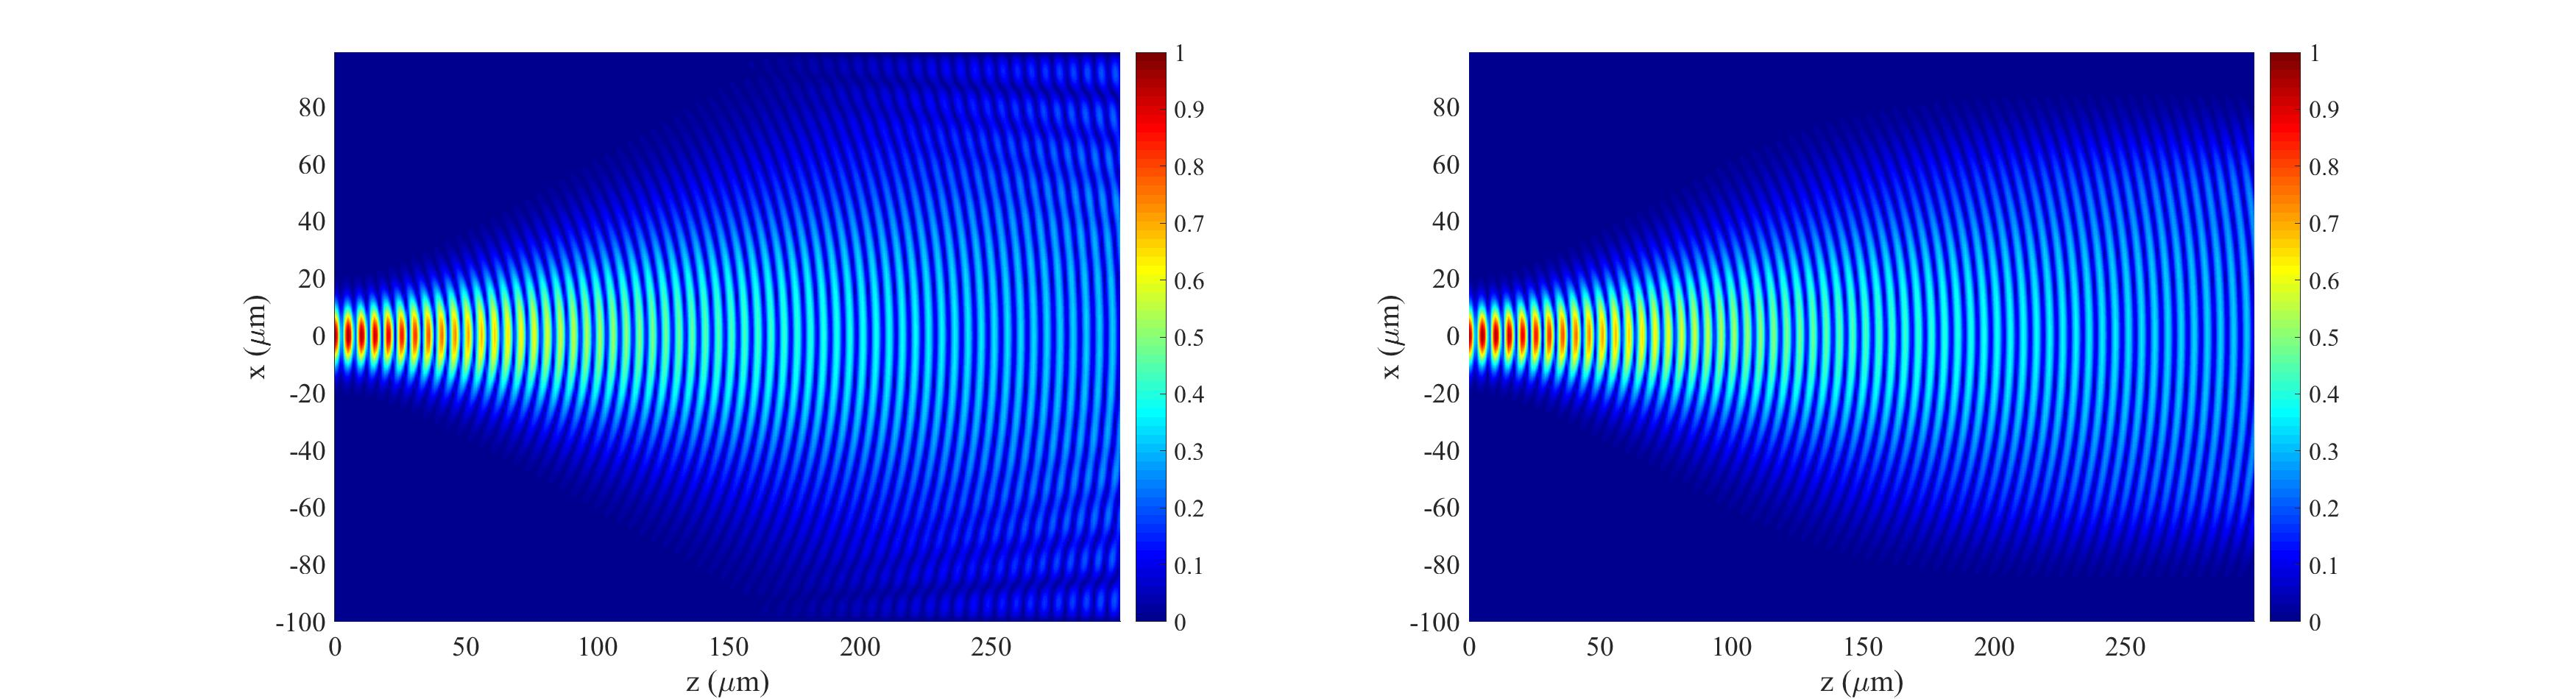
\includegraphics[width=1.5\textwidth]{N3.jpg}
		\caption{\label{fig:Absorption2}Propagation of electric field. On the left implementation of numerical method without ABC, on the right with ABC. Parameters used: z-meshsize = x-meshsize  = 1 $\mu m$, wavelength ($\lambda$) = 10 $\mu m$, waist ($w_o$) = 10 $\mu m$, refractive index ($n_o$) = 1. For ABC simulation $\kappa_{max}$ = 0.0013, $\delta$ =  50 $\mu m$, $l$ = 200 $\mu m$.}
	\end{figure}
	\subsection{X and Z direction meshsize relation}
	In this section we made a research on how x-meshsize and z-meshsize relation affect simulation. In Figure \ref{fig:Relation} change of z-meshsize changes the result of numerical approach. At the point where z-meshsize is equal to x-meshsize numerical method has the most similarity to analytical solution. As result, we can conclude that once one changes x-meshsize, z-meshsize should be changed too and furthermore z-meshsize should be equal to x-meshsize. In the Figure below parameters are: x-meshsize  = 0.5 $\mu m$ is kept constant, wavelength ($\lambda$) = 10 $\mu m$, waist ($w_o$) = 25 $\mu m$, refractive index ($n_o$) = 1, z-meshsize = 1, 0.75, 0.5, 0.375, 0.25 $\mu m$.
%	
	\begin{figure}[H]
		\hspace{-22.5mm}
		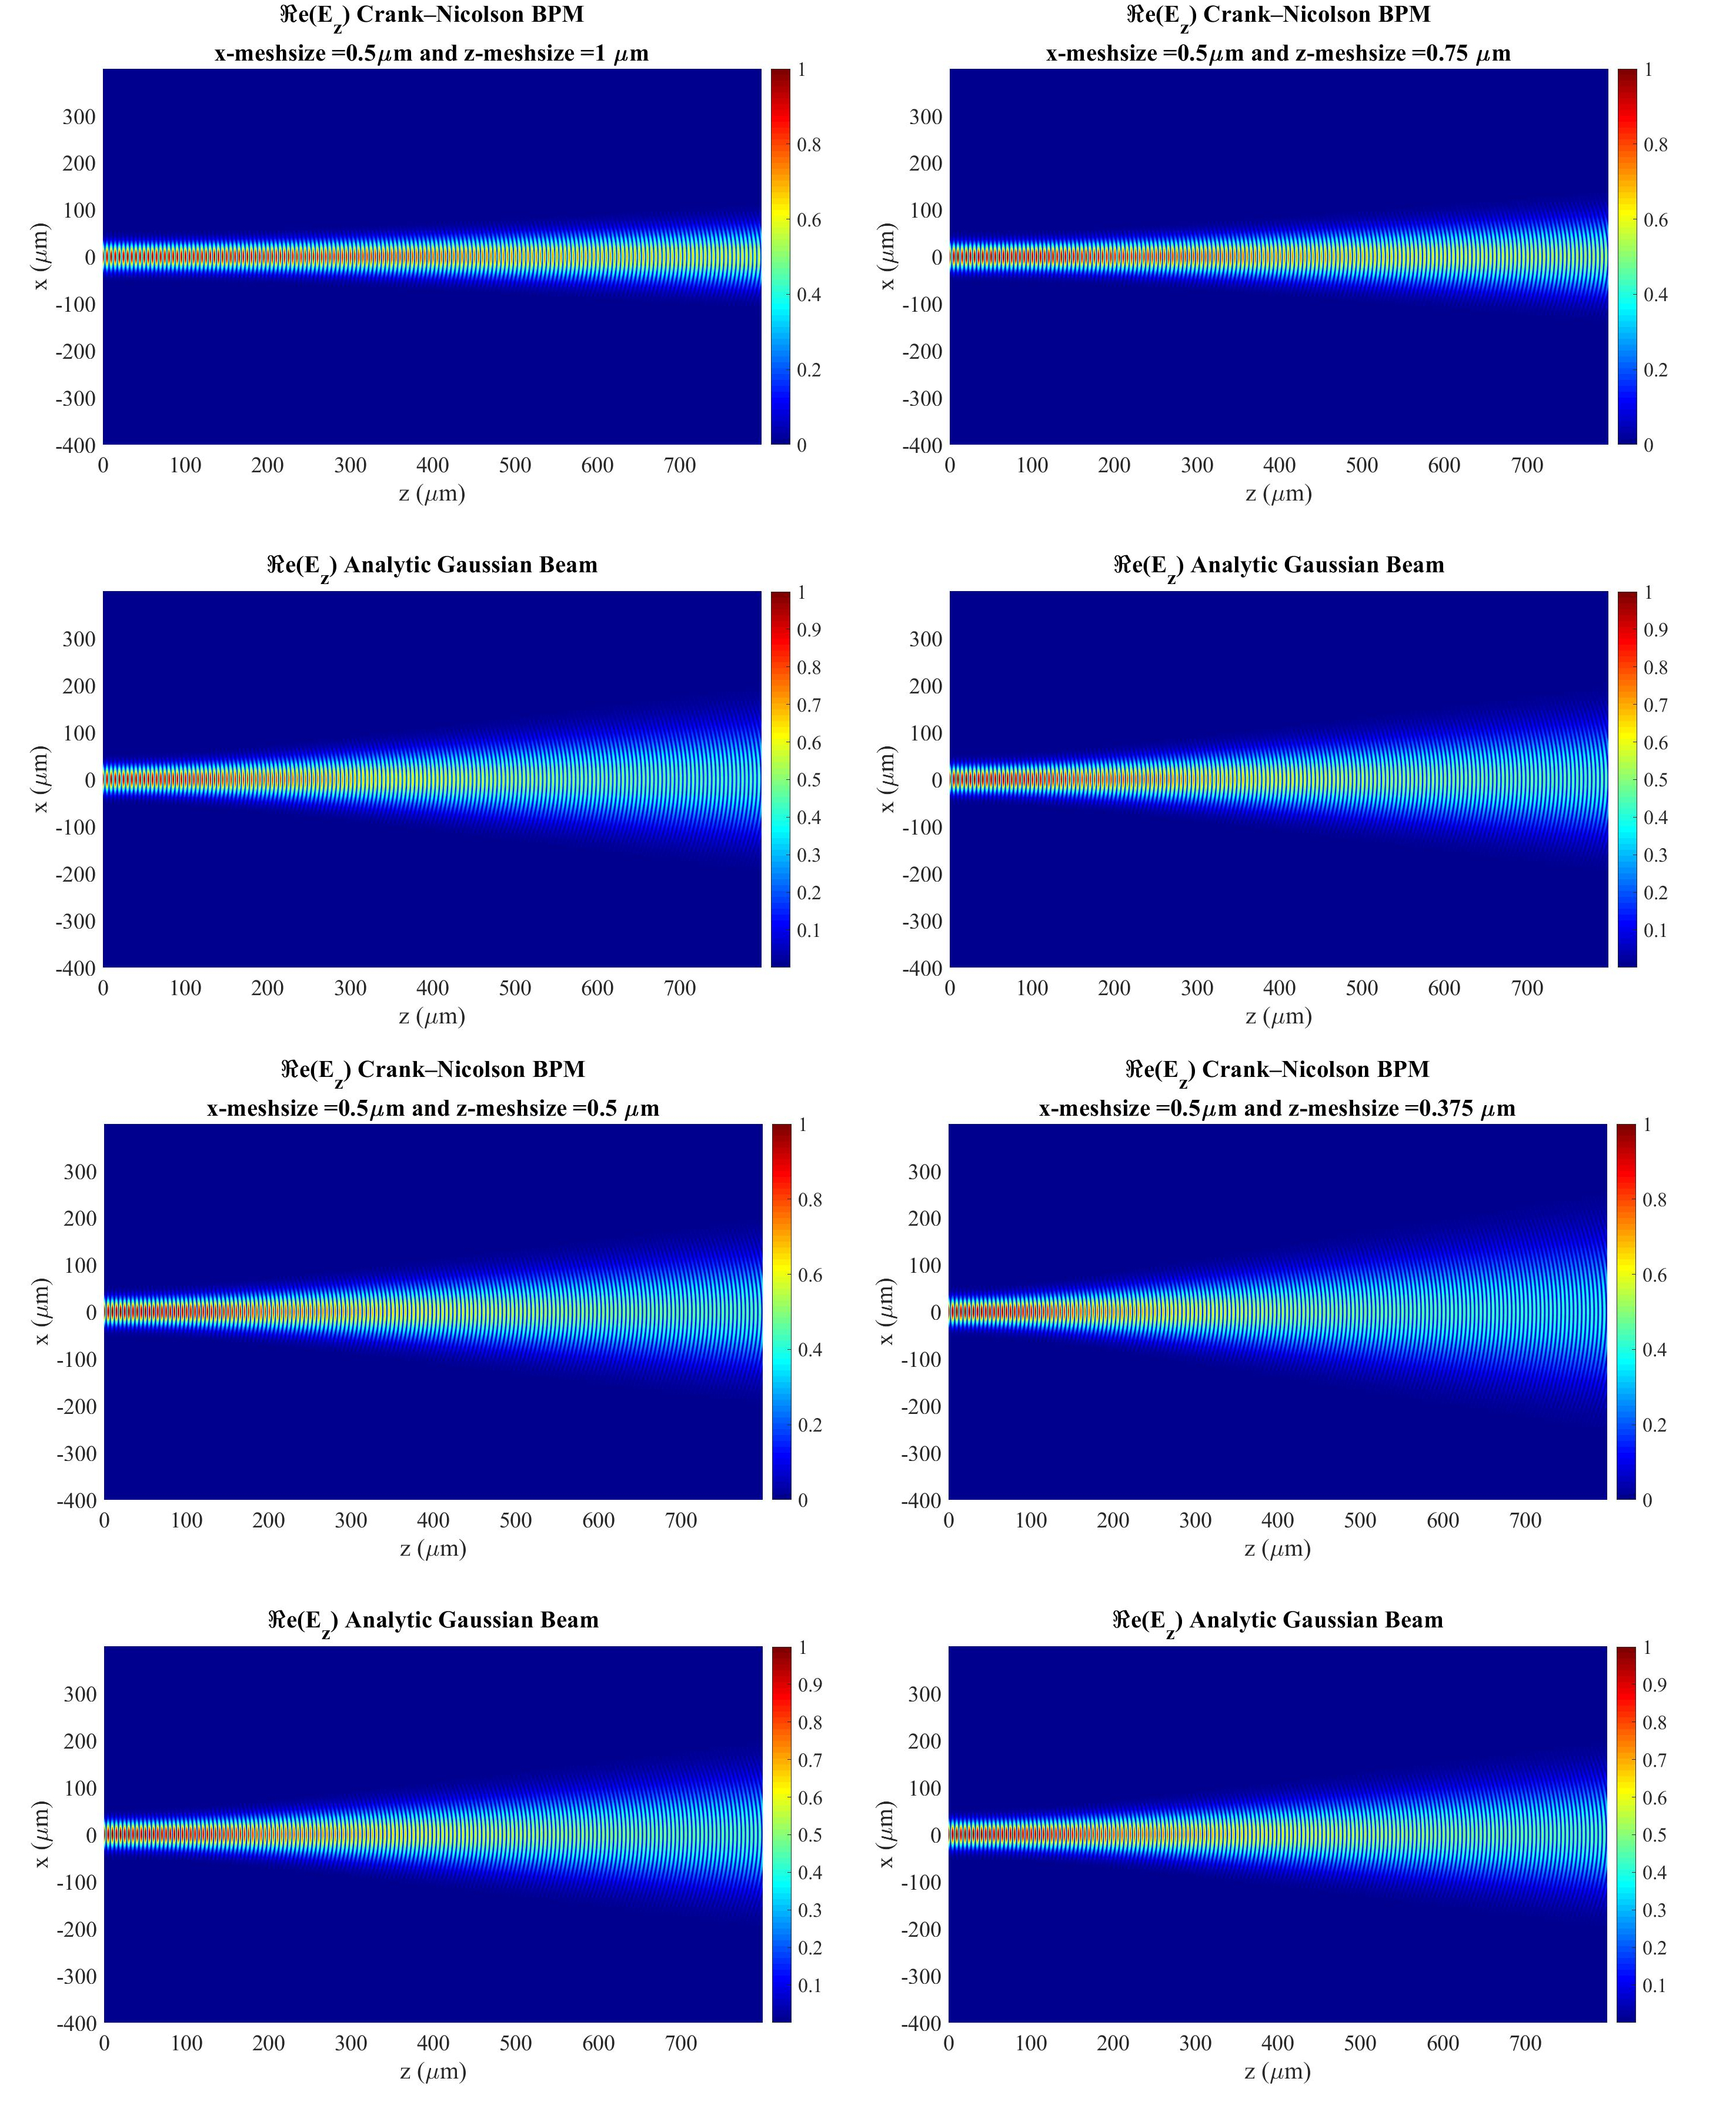
\includegraphics[width=1.35\textwidth]{change1234.jpg}	
	\end{figure}
	
	\begin{figure}[H]
		\hspace{-24.5mm}
		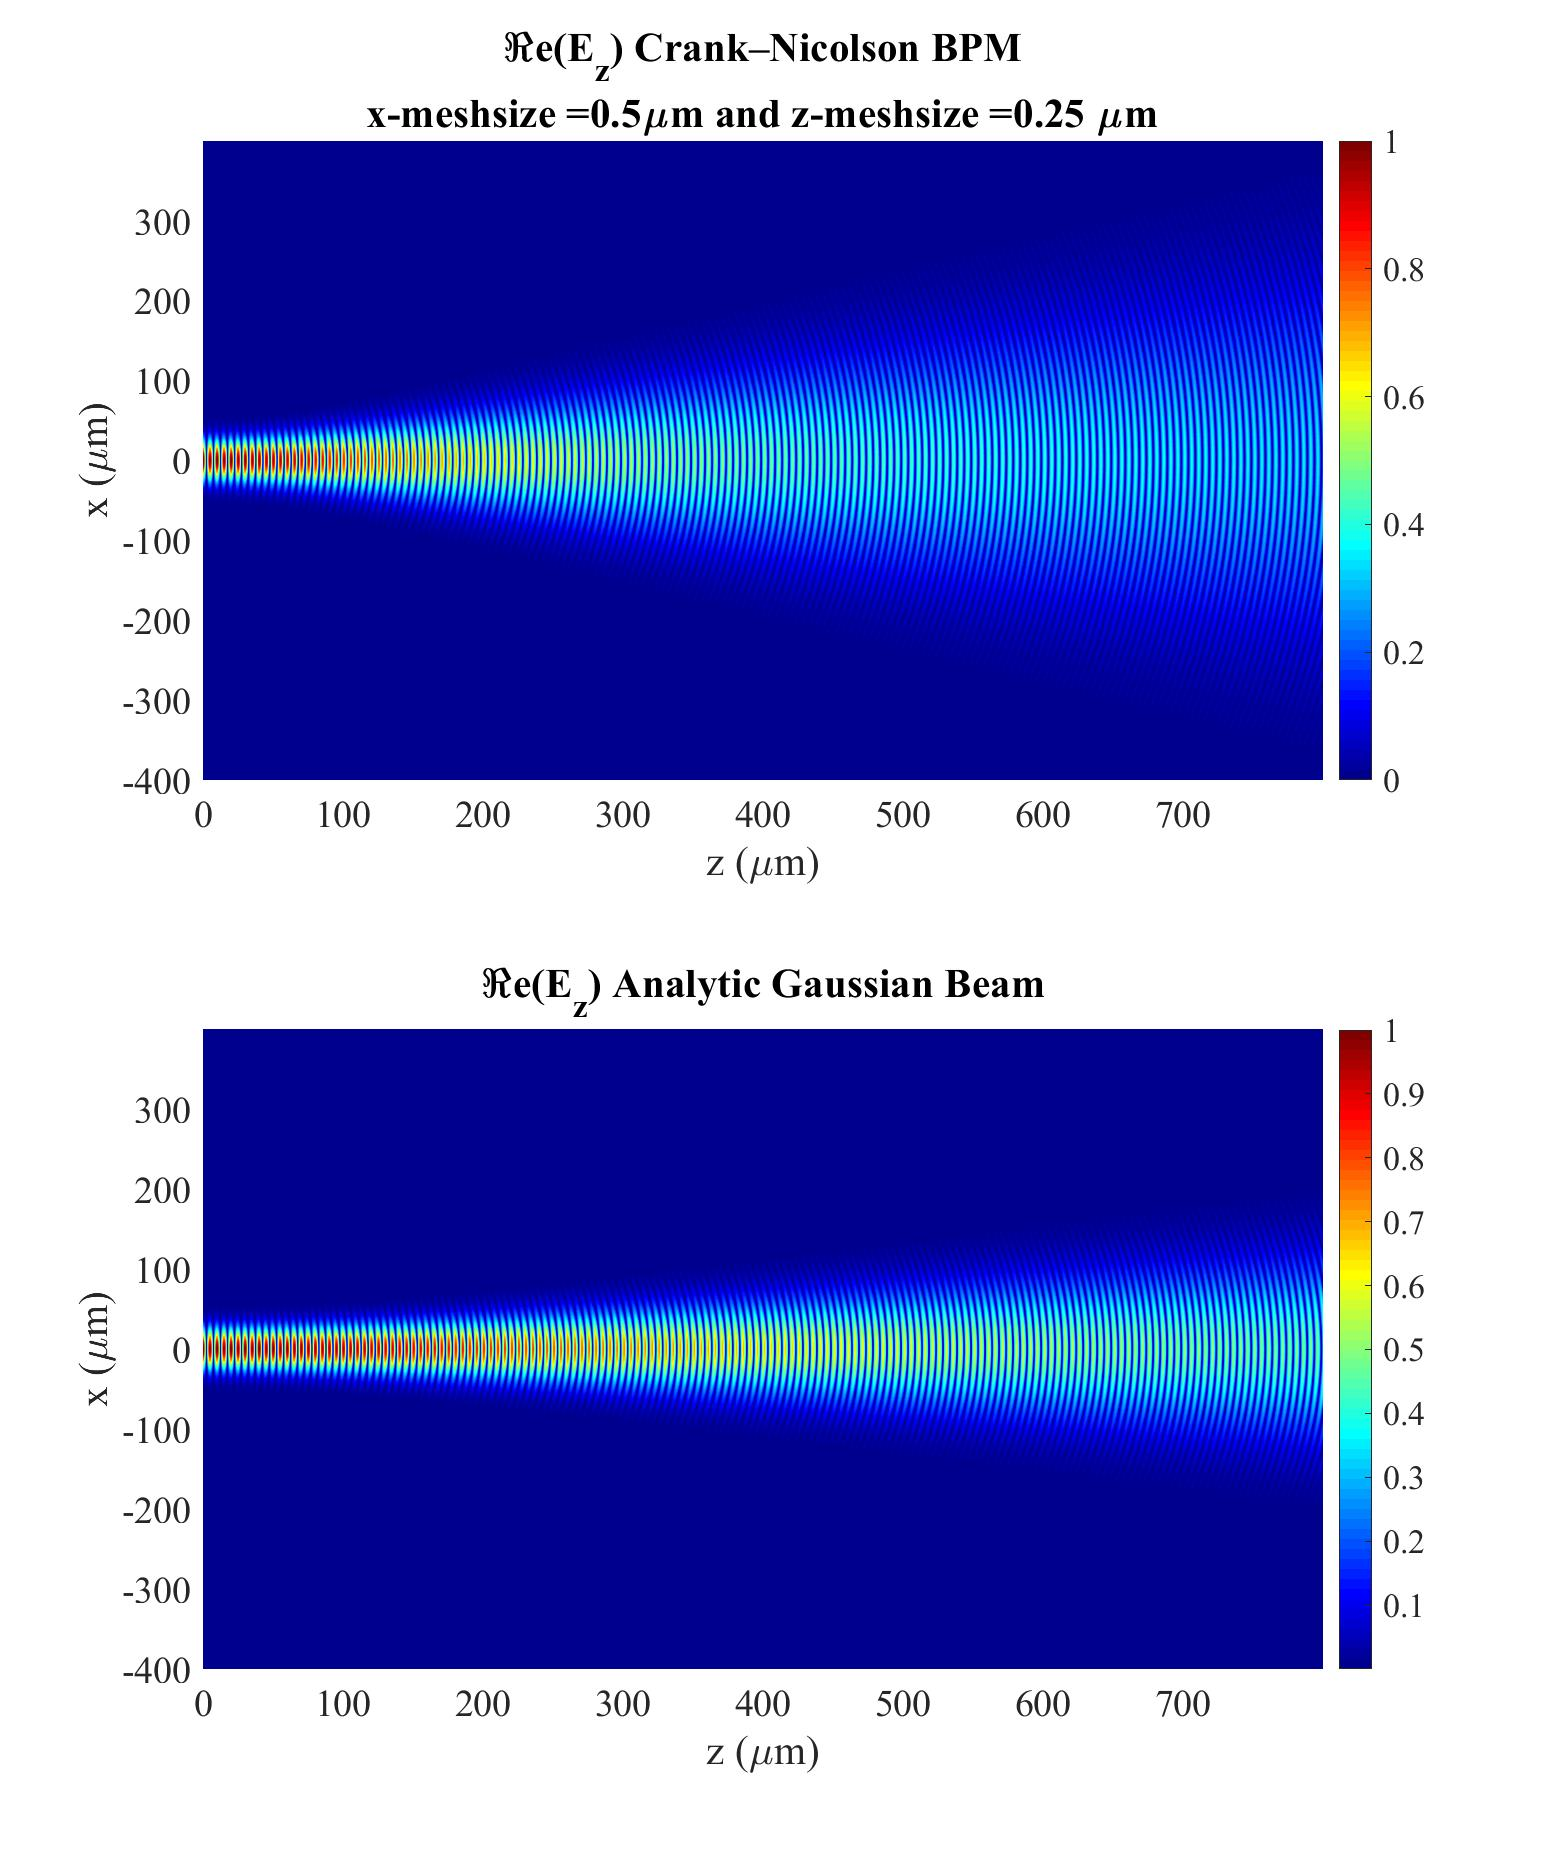
\includegraphics[width=0.725\textwidth]{change5.jpg}	
		\caption{\label{fig:Relation} Numerically computed electric field at different relation of x-meshize and y-meshsize compared to analytical solution.}
	\end{figure}
	
	\subsection{Error convergence}
	In this section error convergence is calculated as described in section 1.2.2, plots are presented in Figure \ref{fig:Error} and results in Table \ref{tab:Table2}. From table we see that if number of grid points increases twice, $L_{2}$ norm error decreases thrice , $L_{\infty}$ increases twice and so on. From Figure we see that of error has steady behavior in logarithmic scale. This convergence is reached at following parameters: wavelength ($\lambda$) = 10 $\mu m$, waist ($w_o$) = 25 $\mu m$, refractive index ($n_o$) = 1, z-meshsize = x-meshsize  = \{2, $\sqrt{2}$, 1, $0.5\sqrt{2}$, 0.5, $0.25\sqrt{2}$, 0.25\} $\mu m$.
	\begin{figure}[H]
		\hspace{-30mm}
		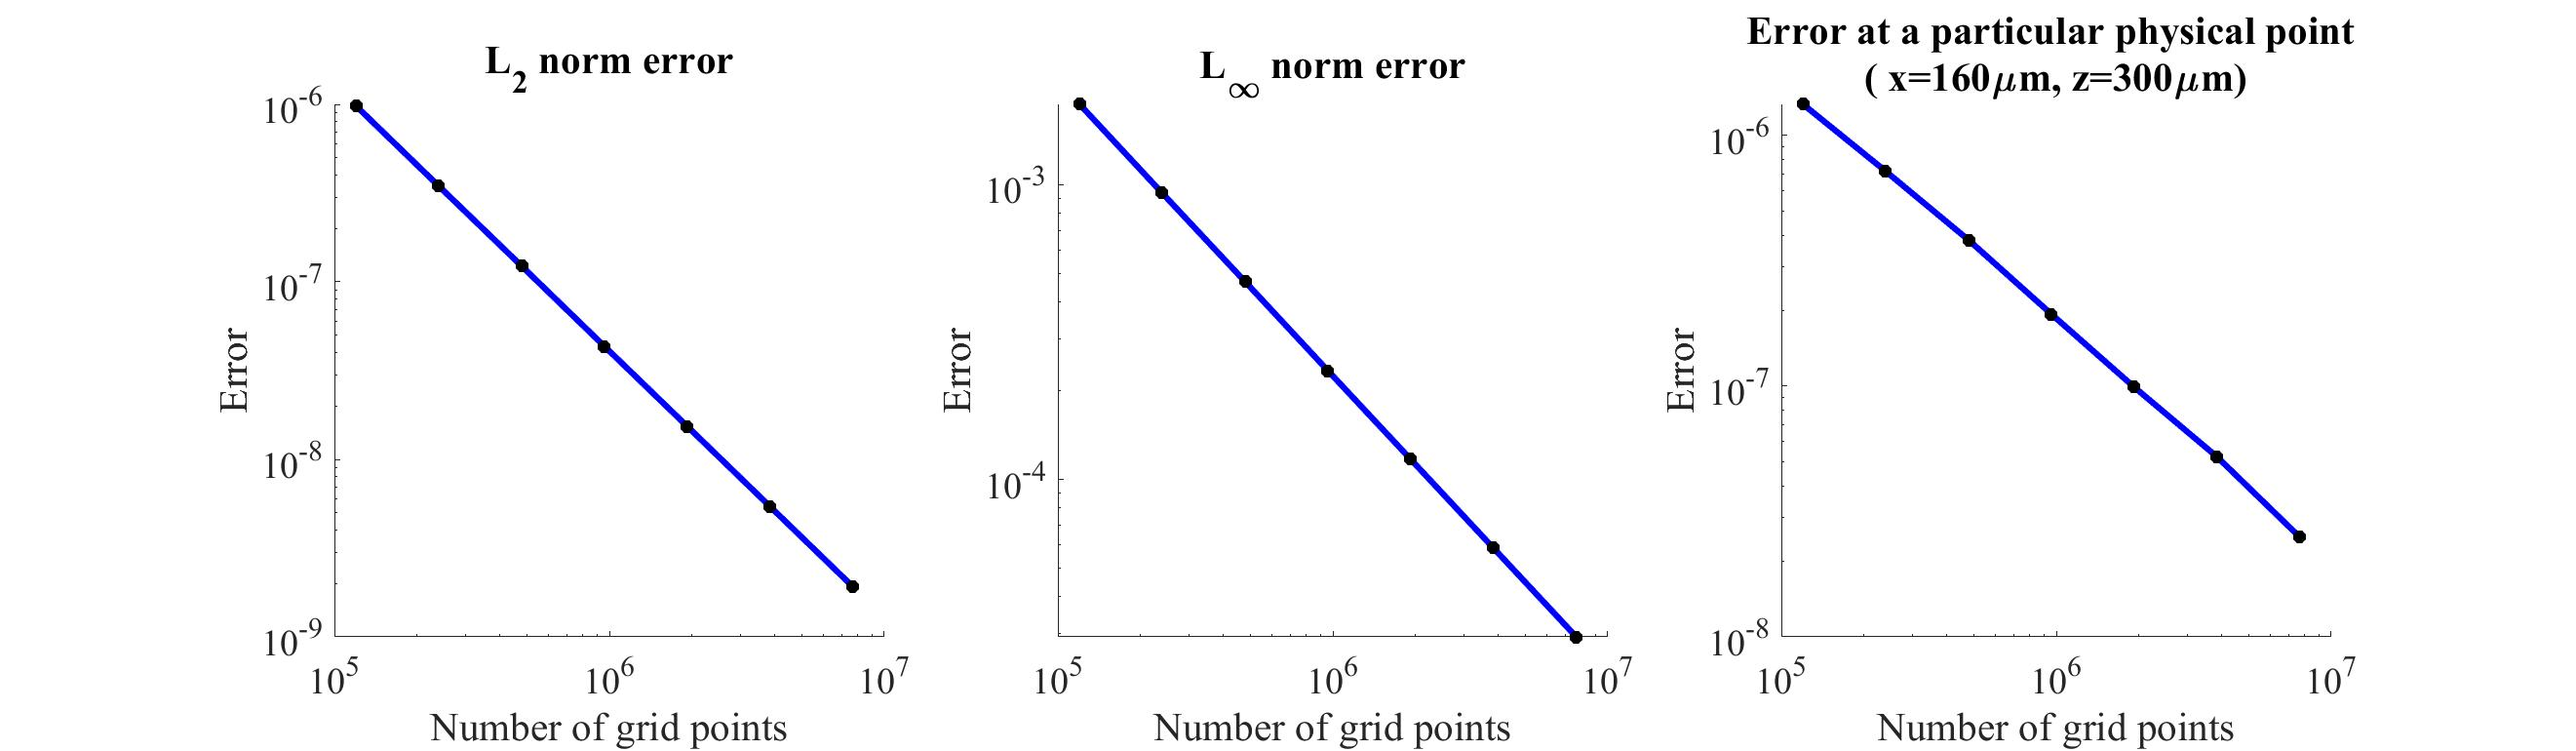
\includegraphics[width=1.5\textwidth]{error.jpg}
		\caption{\label{fig:Error} $L_{2}$, $L_{\infty}$ errors and error at a particular point.}
	\end{figure}
	
	\begin{table}[h!]
		\hspace{-15mm}
		\begin{tabular}{c| c| c| c| c| c| c| c| c} 
			\textbf{ Number of Grid points}& 1 & 2 & 4 & 8 & 16 & 32 & 64 & increase \bf{2x}\\
			\hline
			\textbf{$L_{2}$norm error}& 1 & 0.3546 & 0.1254 & 0.0443 & 0.0156 & 0.0055 & 0.0019& decrease \bf{3x}\\
			\hline
			\textbf{$L_{\infty}$norm error}& 1 & 0.5001 & 0.2503 & 0.1250 & 0.0625 & 0.0312 & 0.0156& decrease \bf{2x}\\
			\hline
			\textbf{Error at a point}& 1 & 0.5410 & 0.2874 & 0.1457 & 0.0745 & 0.0393 & 0.0188& decrease \bf{2x}\\
			
		\end{tabular}
		\caption{\label{tab:Table2}An example table.}
	\end{table}
	
	\newpage
	\section{Conlusion}
	In this report Crank-Nicolson algorithm to simulate Gaussian beam propagation is shown. Results show high resemblance between analytic solution and beam propagation method. In the case when beam propagates in the direction of upper or lower boundary, absorption boundary condition method should be used to compensate the reflection. However in order to keep physical domain same, computational domain should be increased.
	
	\newpage
	
	\section*{Appendix A: ~~Implementation of analytical method}
	\addcontentsline{toc}{section}{Appendix A: Implementation of analytical method}
	\texttt{\noindent
		\textcolor{OliveGreen}{//INITIALIZATION\newline\newline
			// x-coordinate which specifies our computational range in micrometers}.\newline
		x0 = 400 \newline
		\textcolor{OliveGreen}{// meshsize in x-deirection in micrometers.}\newline
		x\_mesh = 1 \newline
		\textcolor{OliveGreen}{// vector which contains x values in micrometers from -x0 to x0 with step x\_mesh.}\newline
		x = from -x0 to x0 with step x\_mesh.\newline
		\textcolor{OliveGreen}{// number of grid points in x-direction.}\newline
		Nx = length(x)\newline
		\textcolor{OliveGreen}{// z-coordinate which specifies our computational range in micrometers.}\newline
		zend = 800 \newline
		\textcolor{OliveGreen}{// meshsize in z-deirection in micrometers.}\newline
		z\_mesh = x\_mesh \newline
		\textcolor{OliveGreen}{// vector which contains z values in micrometers from 0 to zend with step z\_mesh.}\newline
		z = from 0 to zend with step z\_mesh\newline
		\textcolor{OliveGreen}{// number of grid points in z-direction.}\newline
		Nz = length(z)\newline
		\textcolor{OliveGreen}{// waist in micrometers.}\newline
		wo = 30 \newline
		\textcolor{OliveGreen}{// width in micrometers.}\newline
		w = 0 \newline
		\textcolor{OliveGreen}{// curvature in micrometers.}\newline
		r = 0 \newline
		\textcolor{OliveGreen}{// Gouy phase.}\newline
		gouy\_phase = 0 \newline		
		\textcolor{OliveGreen}{// wavelength in micrometers.}\newline
		lambda = 10\newline
		\textcolor{OliveGreen}{// Rayleigh length in micrometers.}\newline
		zR = pi*wo\string^2/lambda;\newline
		\textcolor{OliveGreen}{// refractive index of air in vacuum.}\newline
		no = 1\newline
		\textcolor{OliveGreen}{// spacial frequency with no.}\newline
		ko = 2*pi*no/lambda\newline
		\textcolor{OliveGreen}{// Electic field.}\newline
		E = zeros(Nx,Nz)\newline
		\textcolor{OliveGreen}{// Electic field amplitude.}\newline
		Eo = 1\newline
		\textcolor{OliveGreen}{// 2 dimensional matrix with Nx*Nz size, spacial component of electric field, 2-dimensional grid.}\newpage
		\noindent\textcolor{OliveGreen}{// CORE ALGORITHM}\newline\newline
		\textcolor{OliveGreen}{// Electric field.}\newline
		for i from 1 to Nz \newline
		\indent w = wo*sqrt(1+(z(i)/zR).\string^2);\newline
		\indent r = z(i)+(zR\string^2/z(i));\newline
		\indent gouy\_phase = atan(z(i)/zR);\newline
		\indent E(i\_colomn) = Eo*(wo/w)\string^0.5.*exp(-(x\string^2)/w\string^2) ...\newline \indent\indent\indent\indent\indent\indent\indent\indent*exp(1j*(k*z(i)+k*(x\string^2)/(2*r)-gouy\_phase))\newline
		end for\newline\newline	
	}\newpage
	
	\section*{Appendix B: ~~Implementation of Crank-Nicolson method}
	\addcontentsline{toc}{section}{Appendix B: Implementation of Crank-Nicolson method}
		\texttt{\noindent
			\textcolor{OliveGreen}{// INITIALIZATION\newline\newline
		// x-coordinate which specifies our computational range in micrometers.}\newline
		x0 = 400 \newline
		\textcolor{OliveGreen}{// meshsize in x-deirection in micrometers.}\newline
		x\_mesh = 1 \newline
		\textcolor{OliveGreen}{// vector which contains x values in micrometers from -x0 to x0 with step x\_mesh.}\newline
		x = from -x0 to x0 with step x\_mesh.\newline
		\textcolor{OliveGreen}{// number of grid points in x-direction.}\newline
		Nx = length(x)\newline\newline
		\textcolor{OliveGreen}{// z-coordinate which specifies our computational range in micrometers.}\newline
		zend = 800 \newline
		\textcolor{OliveGreen}{// meshsize in z-deirection in micrometers.}\newline
		z\_mesh = x\_mesh \newline
		\textcolor{OliveGreen}{// vector which contains z values in micrometers from 0 to zend with step z\_mesh.}\newline
		z = from 0 to zend with step z\_mesh\newline
		\textcolor{OliveGreen}{// number of grid points in z-direction.}\newline
		Nz = length(z)\newline
		\textcolor{OliveGreen}{// waist in micrometers.}\newline
		wo = 30 \newline
		\textcolor{OliveGreen}{// wavelength in micrometers.}\newline
		lambda = 10\newline
		\textcolor{OliveGreen}{// refractive index of air in vacuum.}\newline
		no = 1\newline
		\textcolor{OliveGreen}{// spacial frequency with no.}\newline
		ko = 2*pi*no/lambda\newline
		\textcolor{OliveGreen}{// refractive index of medium.}\newline
		n = 1\newline
		\textcolor{OliveGreen}{// spacial frequency with n.}\newline
		k = 2*pi*n/lambda\newline\newline
		\textcolor{OliveGreen}{// 2 dimensional matrix with Nx*Nz size, complete electric field, 2-dimensional grid.}\newline
		E = zeros(Nx,Nz)\newline
		\textcolor{OliveGreen}{// 2 dimensional matrix with Nx*Nz size, spacial component of electric field, 2-dimensional grid.}\newline
		u = zeros(Nx,Nz)\newline
		\textcolor{OliveGreen}{// 2 dimensional matrix with Nx*Nz size, periodic component of electric field in z direction, 2-dimensional grid.}\newline
		f = zeros(Nx,Nz)\newline
		\textcolor{OliveGreen}{// 2 dimensional matrix with Nx*Nx size, tridiagonal matrix or Thomas algorithm (see section 1.2).}\newline
		L = zeros(Nx,Nx)\newline
		\textcolor{OliveGreen}{// 2 dimensional matrix with Nx*Nx size, identity matrix used in Thomas algorithm.}\newline
		I = eye(Nx,Nx)\newline\newline
		\textcolor{OliveGreen}{// set first colomn of u to gaussian.}\newline
		u(first\_colomn) = exp(-(x/wo)\string^2)\newline\newline
		\textcolor{OliveGreen}{// CORE ALGORITHM}\newline\newline
		\textcolor{OliveGreen}{// L matrix computation.}\newline
		for i from 1 to Nx \newline
		\indent L(i,i) = 1/x\_mesh\string^2*(-2+(ko\string^2-k\string^2)*x\_mesh\string^2)\newline
		\indent if i>1\newline
		\indent\indent L(i,i-1)=1/x\_mesh\string^2\newline
		\indent\indent L(i-1,i)=1/x\_mesh\string^2\newline
		\indent end if\newline
		end for\newline\newline	
		\textcolor{OliveGreen}{// Spacial component of electric field computation.}\newline
		for i\_colomn from 2 to Nz\newline
		\indent u(i\_colomn) = MatrixInverse(I-x\_mesh*L/(4*1j*ko))*...\newline
		\indent\indent\indent\indent\indent\indent\indent\indent\indent\indent\indent(E+x\_mesh*L/(4*1j*ko)))*u(i\_colomn-1)\newline
		end for\newline\newline
		\textcolor{OliveGreen}{// Periodic component of electric field in z direction computation.}\newline
		for i\_colomn from 1 to Nz\newline
		\indent f(i\_colomn) = exp(-1j*ko*z(i\_colomn))\newline
		end for\newline\newline
		\textcolor{OliveGreen}{// Complete Electric field.}\newline
		E = Elementwise\_multiplication(u,f)\newline\newline
	    }
		\newpage

	
		
\end{document}




